\documentclass[10pt]{beamer}
\usetheme[
%%% option passed to the outer theme
%    progressstyle=fixedCircCnt,   % fixedCircCnt, movingCircCnt (moving is deault)
  ]{Feather}
%-------------------------------------------------------
% INCLUDE PACKAGES
%-------------------------------------------------------

\usepackage[utf8]{inputenc}
\usepackage[english]{babel}
\usepackage[T1]{fontenc}
\usepackage{helvet}


%-------------------------------------------------------
% Hack for hyperref warnings from the pdflatex compiler
%-------------------------------------------------------
\pdfstringdefDisableCommands{%
  \def\\{}%
}

%-------------------------------------------------------
% DEFFINING AND REDEFINING COMMANDS
%-------------------------------------------------------

% colored hyperlinks
\newcommand{\chref}[2]{
  \href{#1}{{\usebeamercolor[bg]{Feather}#2}}
}

%-------------------------------------------------------
% INFORMATION IN THE TITLE PAGE
%-------------------------------------------------------

\title[Religion, Meet Science] % [] is optional - is placed on the bottom of the sidebar on every slide
{ % is placed on the title page
      \textbf{Religion, Meet Science}
}

\subtitle{\textit{(Chapter 3)}}

\author{
	Brennan Fieck, Brionna Dumlao\\
    Nathan Fishel, Erin Hamand \\
    Kendyll Hawkins, Kris Lide \\
	Matthew McDonald, Zacary Parkhill
}

\date{\today}

%-------------------------------------------------------
% THE BODY OF THE PRESENTATION
%-------------------------------------------------------

\begin{document}

%-------------------------------------------------------
% THE TITLEPAGE
%-------------------------------------------------------

{\1% % this is the name of the PDF file for the background
\begin{frame}[plain,noframenumbering] % the plain option removes the header from the title page, noframenumbering removes the numbering of this frame only
  \titlepage % call the title page information from above
\end{frame}}

%Sections 1 & 2
%-------------------------------------------------------
\section{In the Beginning}
\subsection{The United States}
%-------------------------------------------------------
\begin{frame}{In the Beginning}{The United States}
%-------------------------------------------------------
	\begin{itemize}
		\item<1 -> Settled by Christians - the Puritans.
		\item<2 -> Founded on science - logic and reason.
			\begin{itemize}
				\item<3 -> Logic and reason helped ensure religious freedom
				\item<3 -> This is why religious mentality was not incorporated into the Declaration of Independence
			\end{itemize}
	\end{itemize}
\end{frame}

%-------------------------------------------------------
\subsection{God's Natural Law is Reason}
%-------------------------------------------------------
\begin{frame}{In the Beginning}{God's Natural Law is Reason}
%-------------------------------------------------------
	\begin{columns}[T]
		\column{0.6\textwidth}
			From approx. 700 C.E. to 900 C.E.\\
			\begin{itemize}
				\item Mu'tazilites mode of study
					\begin{itemize}
						\item Discern God's will by studying nature
						\item God speaks through nature
					\end{itemize}
			\end{itemize}
		\column{0.4\textwidth}
			\begin{figure}
				\centering
				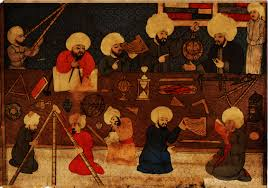
\includegraphics[width=\textwidth]{images/mutazilite_science}
				\caption{Mu'tazilite Science}
			\end{figure}
	\end{columns}
\end{frame}

%-------------------------------------------------------
\begin{frame}{In the Beginning}{God's Natural Law is Reason}
%-------------------------------------------------------
	\begin{columns}[T]
		\column{0.6\textwidth}
			1517 C.E.
			\begin{itemize}
				\item Martin Luther nails his 95 theses to the door of a Catholic church to protest the Church's practices
					\begin{itemize}
						\item Protestants argued that knowledge comes from observing God's Word, not the Pope's word
					\end{itemize}
			\end{itemize}
		\column{0.4\textwidth}
			\begin{figure}
				\centering
				
\includegraphics[width=\textwidth]{images/martin_luther}
				\caption{Martin Luther}
			\end{figure}
	\end{columns}
\end{frame}

%-------------------------------------------------------
\begin{frame}{In the Beginning}{God's Natural Law is Reason}
%-------------------------------------------------------
	\begin{columns}[T]
		\column{0.6\textwidth}
			1518 C.E.
			\begin{itemize}
				\item Protestant polemicist St. Germain supports "do it yourself" Bible study
					\begin{itemize}
						\item Protestants argued that knowledge comes from observing God's Word, not the Pope's word
						\item Use one's own experience of the Bible to find truth\\
							This approach is in the same "anti-authoritarian" vein as the modern scientific approach (make observations, then come to conclusions)
					\end{itemize}
			\end{itemize}
		\column{0.4\textwidth}
			\begin{figure}
				\centering
				
\includegraphics[width=\textwidth]{images/martin_luther}
				\caption{Martin Luther}
			\end{figure}
	\end{columns}
\end{frame}

%-------------------------------------------------------
\begin{frame}{In the Beginning}{God's Natural Law is Reason}
%-------------------------------------------------------
	\begin{columns}[T]
		\column{0.6\textwidth}
			Early 1600's
			\begin{itemize}
				\item Puritan sympathizer Edward Coke argues that scientific laws could be studied by everyone, and could not be overruled by the crown.
			\end{itemize}
		\column{0.4\textwidth}
			\begin{figure}
				\centering
				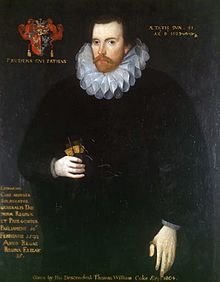
\includegraphics[width=\textwidth]{images/edward_coke}
				\caption{Edward Coke}
			\end{figure}
	\end{columns}
\end{frame}

%-------------------------------------------------------
\begin{frame}{In the Beginning}{God's Natural Law is Reason}
%-------------------------------------------------------
	\begin{columns}[T]
		\column{0.6\textwidth}
			Late 1500's to mid 1600's
			\begin{itemize}
				\item Puritans supported a logical, antiauthoritarian approach to theology:
					\begin{itemize}
						\item Making your own observations from the Bible and not relying on the Pope
						\item Use observations to draw broader theological conclusions
						\item Puritans study Mu'tazilite science books
					\end{itemize}
			\end{itemize}
		\column{0.4\textwidth}
			\begin{figure}
				\centering
				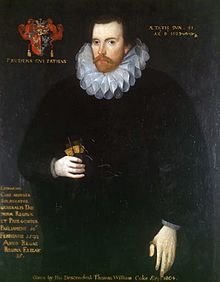
\includegraphics[width=\textwidth]{images/edward_coke.png}
				\caption{Edward Coke}
			\end{figure}
	\end{columns}
\end{frame}



% Timeline of Events:

% ~A.D. 700-900: Mu’tazilites mode of study: Discern God’s will by studying nature
% God speaks through nature
% 1517: Beginning of the Protestant Reformation 
% Martin Luther nails his 95 Theses, in protest of the Catholic Church’s practices
% Protestants argued that knowledge comes from observing God’s Word, not the Pope’s word
% 1518: Protestant polemicist St. Germain supports “do it yourself” Bible study
%           - Use one own’s experience of the Bible to find truth
%           - This approach used was of the same “antiauthoritarian” nature of the emerging (now modern) scientific approach (make observations, then come to conclusion)

% Early 1600s: Puritan sympathizer Edward Coke argues that scientific laws could be studied by everyone, and could not be overruled by the crown.

% Late 1500s to mid-1600s:  Puritans supported a logical, antiauthoritarian approach to theology:
% Making your own observations from the Bible and not relying on the Pope
% Use observations to draw broader theological conclusions
% Puritans study Mu’tazilite science books


%Section 4
%-------------------------------------------------------
\section{The DNA of Western Thought}
%-------------------------------------------------------
\begin{frame}{The DNA of Western Thought}{}
%-------------------------------------------------------
	Western Christianity is composed of two main groups:
	\begin{enumerate}
		\item Roman Catholicism
		\item Protestantism
	\end{enumerate}
\end{frame}


%Section 5
%-------------------------------------------------------
\section{Descartes vs. Bacon}
\subsection{Descartes}
%-------------------------------------------------------
\begin{frame}{Descartes vs. Bacon}{Descartes}
%-------------------------------------------------------
	Descartes focused on the "mind-body split"
	\begin{itemize}
		\item Said that conclusions are only valid if they follow logically from the premise
		\item "I think therefore I am" - \textit{Renee Descartes}
		\item Wanted to embrace skepticism
		\item Said that senses are unreliable and a source of untruth and illusion\\
			Only reliable from a mind that was separate from the body
	\end{itemize}
\end{frame}

%-------------------------------------------------------
\subsection{Bacon}
%-------------------------------------------------------
\begin{frame}{Descartes vs. Bacon}{Bacon}
%-------------------------------------------------------
	Bacon focused on science and published a "New Instrument of Science"
	\begin{itemize}
		\item Inductive reasoning -\\
			From bottom up, observing with senses and then building logical steps to reach a general conclusion about reality
		\item His method is "Flawed" because conclusions are provisional and leave room to be disproved
	\end{itemize}
	Bacon's method is good for science because it
	\begin{itemize}
		\item contains a provisional "probably" statement
		\item shows how math and science have become important, quantifies whether a relative probability is T/F
	\end{itemize}
\end{frame}


%Section 6
%-------------------------------------------------------
\section{Puritan Science}
\subsection{Francis Bacon}
%-------------------------------------------------------
\begin{frame}{Puritan Science}{Francis Bacon}
%-------------------------------------------------------
	Francis Bacon's method of scientific thought states that Conclusions are made because they are supported by all the facts observed so far. This is very similar to the Puritan method of thinking regarding philosophy and religion.
\end{frame}

%-------------------------------------------------------
\subsection{Puritan Frustrations}
%-------------------------------------------------------
\begin{frame}{Puritan Science}{Puritan Frustrations}
%-------------------------------------------------------
	\begin{itemize}
		\item Since Protestantism was a protest against Catholic authority, Puritans disliked Catholic indictments or Christian fundamentalism.
			\begin{itemize}
				\item Indictment of Galileo
				\item Disliked denial of opinions supported by observation of nature, therefore evidence of God's will, because it conflicted with scripture
			\end{itemize}
		\item Believed the Church of England was too Catholic
			\begin{itemize}
				\item Demanded a new translation of the Bible in 1604 (the "King James" version)
				\item Believed having a monarch that was also the head of a church was incompatible and hypocritically self-serving
			\end{itemize}
		\item King Charles I's reintroduction of Catholicism to England and similar absolutism behavior led to Puritan migration to America
	\end{itemize}
\end{frame}

%-------------------------------------------------------
\subsection{Puritan and Anti-Authoritarian Influence in America}
%-------------------------------------------------------
\begin{frame}{Puritan Science}{Puritan and Anti-Authoritarian Influence in America}
%-------------------------------------------------------
	\begin{itemize}
		\item Edward Coke
			\begin{itemize}
				\item While in Parliament he attempted to limit the king's powers, including writing the Petition of Right, which laid out these basic rights the US would later adopt:
				\begin{enumerate}
					\item Taxes levied only by Parliament not by the king
					\item No martial law in peacetime
					\item Soldiers could not be forcibly housed by civilians
				\end{enumerate}
				\item Influenced the English Civil Wars and led to the Restoration of the Church of England and tolerated Puritanism\\
					Due to Puritanism encouraging individual liberty, many great scientists were members
			\end{itemize}
		\item Isaac Newton
			\begin{itemize}
				\item Wrote \textit{Mathematical Principles of Natural Philosophy}
				\item Influenced Thomas Jefferson's writing in the Declaration of Independence
			\end{itemize}
	\end{itemize}
\end{frame}


%Section 7
%-------------------------------------------------------
\section{The Sciencist-Politician}
%-------------------------------------------------------
\begin{frame}{The Sciencist-Politician}{Thomas Jefferson}
%-------------------------------------------------------
	\begin{itemize}
		\item Appointed by the Continental Congress to draft the Declaration of Independence, Jefferson was heavily influenced by Isaac Newton and Edward Coke's writings to establish:
			\begin{itemize}
				\item A limit on the power of a monarch by writing a document for the US that was based on knowledge and reason, not God
				\item A country based on the rule of men, a democracy, which would be appealing to people of all religions and denominations as one would not have power over the others
			\end{itemize}
		\item As president he commissioned the Lewis and Clark expedition. He received support for it from Congress by presenting it as an economic initiative, but in reality he ordered Lewis to undergo the journey as though it were a scientific expedition.
	\end{itemize}
\end{frame}


%-------------------------------------------------------
\section{How Do We Know Things?}
%-------------------------------------------------------
\begin{frame}{How Do We \textit{Know} Things?}{(auth. Brennan Fieck)}
%-------------------------------------------------------

  \begin{itemize}
    \item The Feather image is not covered by copyright rules. I have used the image from \chref{http://www.vectors-free.com/}{http://www.vectors-free.com/}. You are allowed to use the Feather image for any purposes.
    \item The rest of the theme is provided under the GNU General Public License v. 3 (GPLv3) \chref{http://www.gnu.org/licenses/}{http://www.gnu.org/licenses/}. This means that you can redistribute it and/or modify it under the same license. 
  \end{itemize}
\end{frame}

\end{document}